\chapter{SupleMentor - Um Assistente Especialista em Suplementação Esportiva}

\begin{flushright}
Adrian Trajano de Almeida da Silva
\end{flushright}

O SupleMentor é um Assistente Virtual Especialista em suplementação esportiva e nutrição voltada ao auxílio de praticantes de exercícios físicos. Seu objetivo é ajudar tanto praticantes de atividades físicas como interessados no tema a compreender o funcionamento, as dosagens de referência, os horários adequados e as restrições de segurança dos principais suplementos alimentares.

Com a popularização de rotinas de treino e o fácil acesso a suplementos comerciais, cresce também a circulação de informações imprecisas e recomendações sem respaldo técnico, o que pode gerar desde gastos desnecessários até riscos à saúde de pessoas com condições específicas, como hipertensão ou intolerância à lactose. Nesse cenário, a integração entre Grandes Modelos de Linguagem (LLMs) e técnicas de Sistemas Especialistas permite combinar a fluidez conversacional com conhecimento estruturado e raciocínio controlado por regras \cite{yang2025comprehensive, garridomerchan2026gofai}.

O desenvolvimento do SupleMentor aplica essa abordagem ao disponibilizar uma interface conversacional contextualizada por persona, apoiada por uma base de conhecimento própria, um cache semântico em banco vetorial e um servidor de ferramentas especialistas via \textit{Model Context Protocol} (MCP). As seções seguintes detalham a arquitetura, as ferramentas MCP, o desenvolvimento com avaliação automatizada e os recursos de reprodutibilidade da solução.

\section{Arquitetura do SupleMentor}

A Figura \ref{fig:arquitetura-suplementor} apresenta a arquitetura de componentes do SupleMentor. O usuário interage com o sistema por meio de uma interface de chat, implementada tanto em ambiente web (via \textit{Streamlit}, exibindo telemetria de sessão em tempo real) quanto em linha de comando (terminal). Cada pergunta enviada é recebida pelo núcleo do Sistema Especialista antes de acionar a inferência do modelo generativo.

\begin{figure}[htbp]
\centering
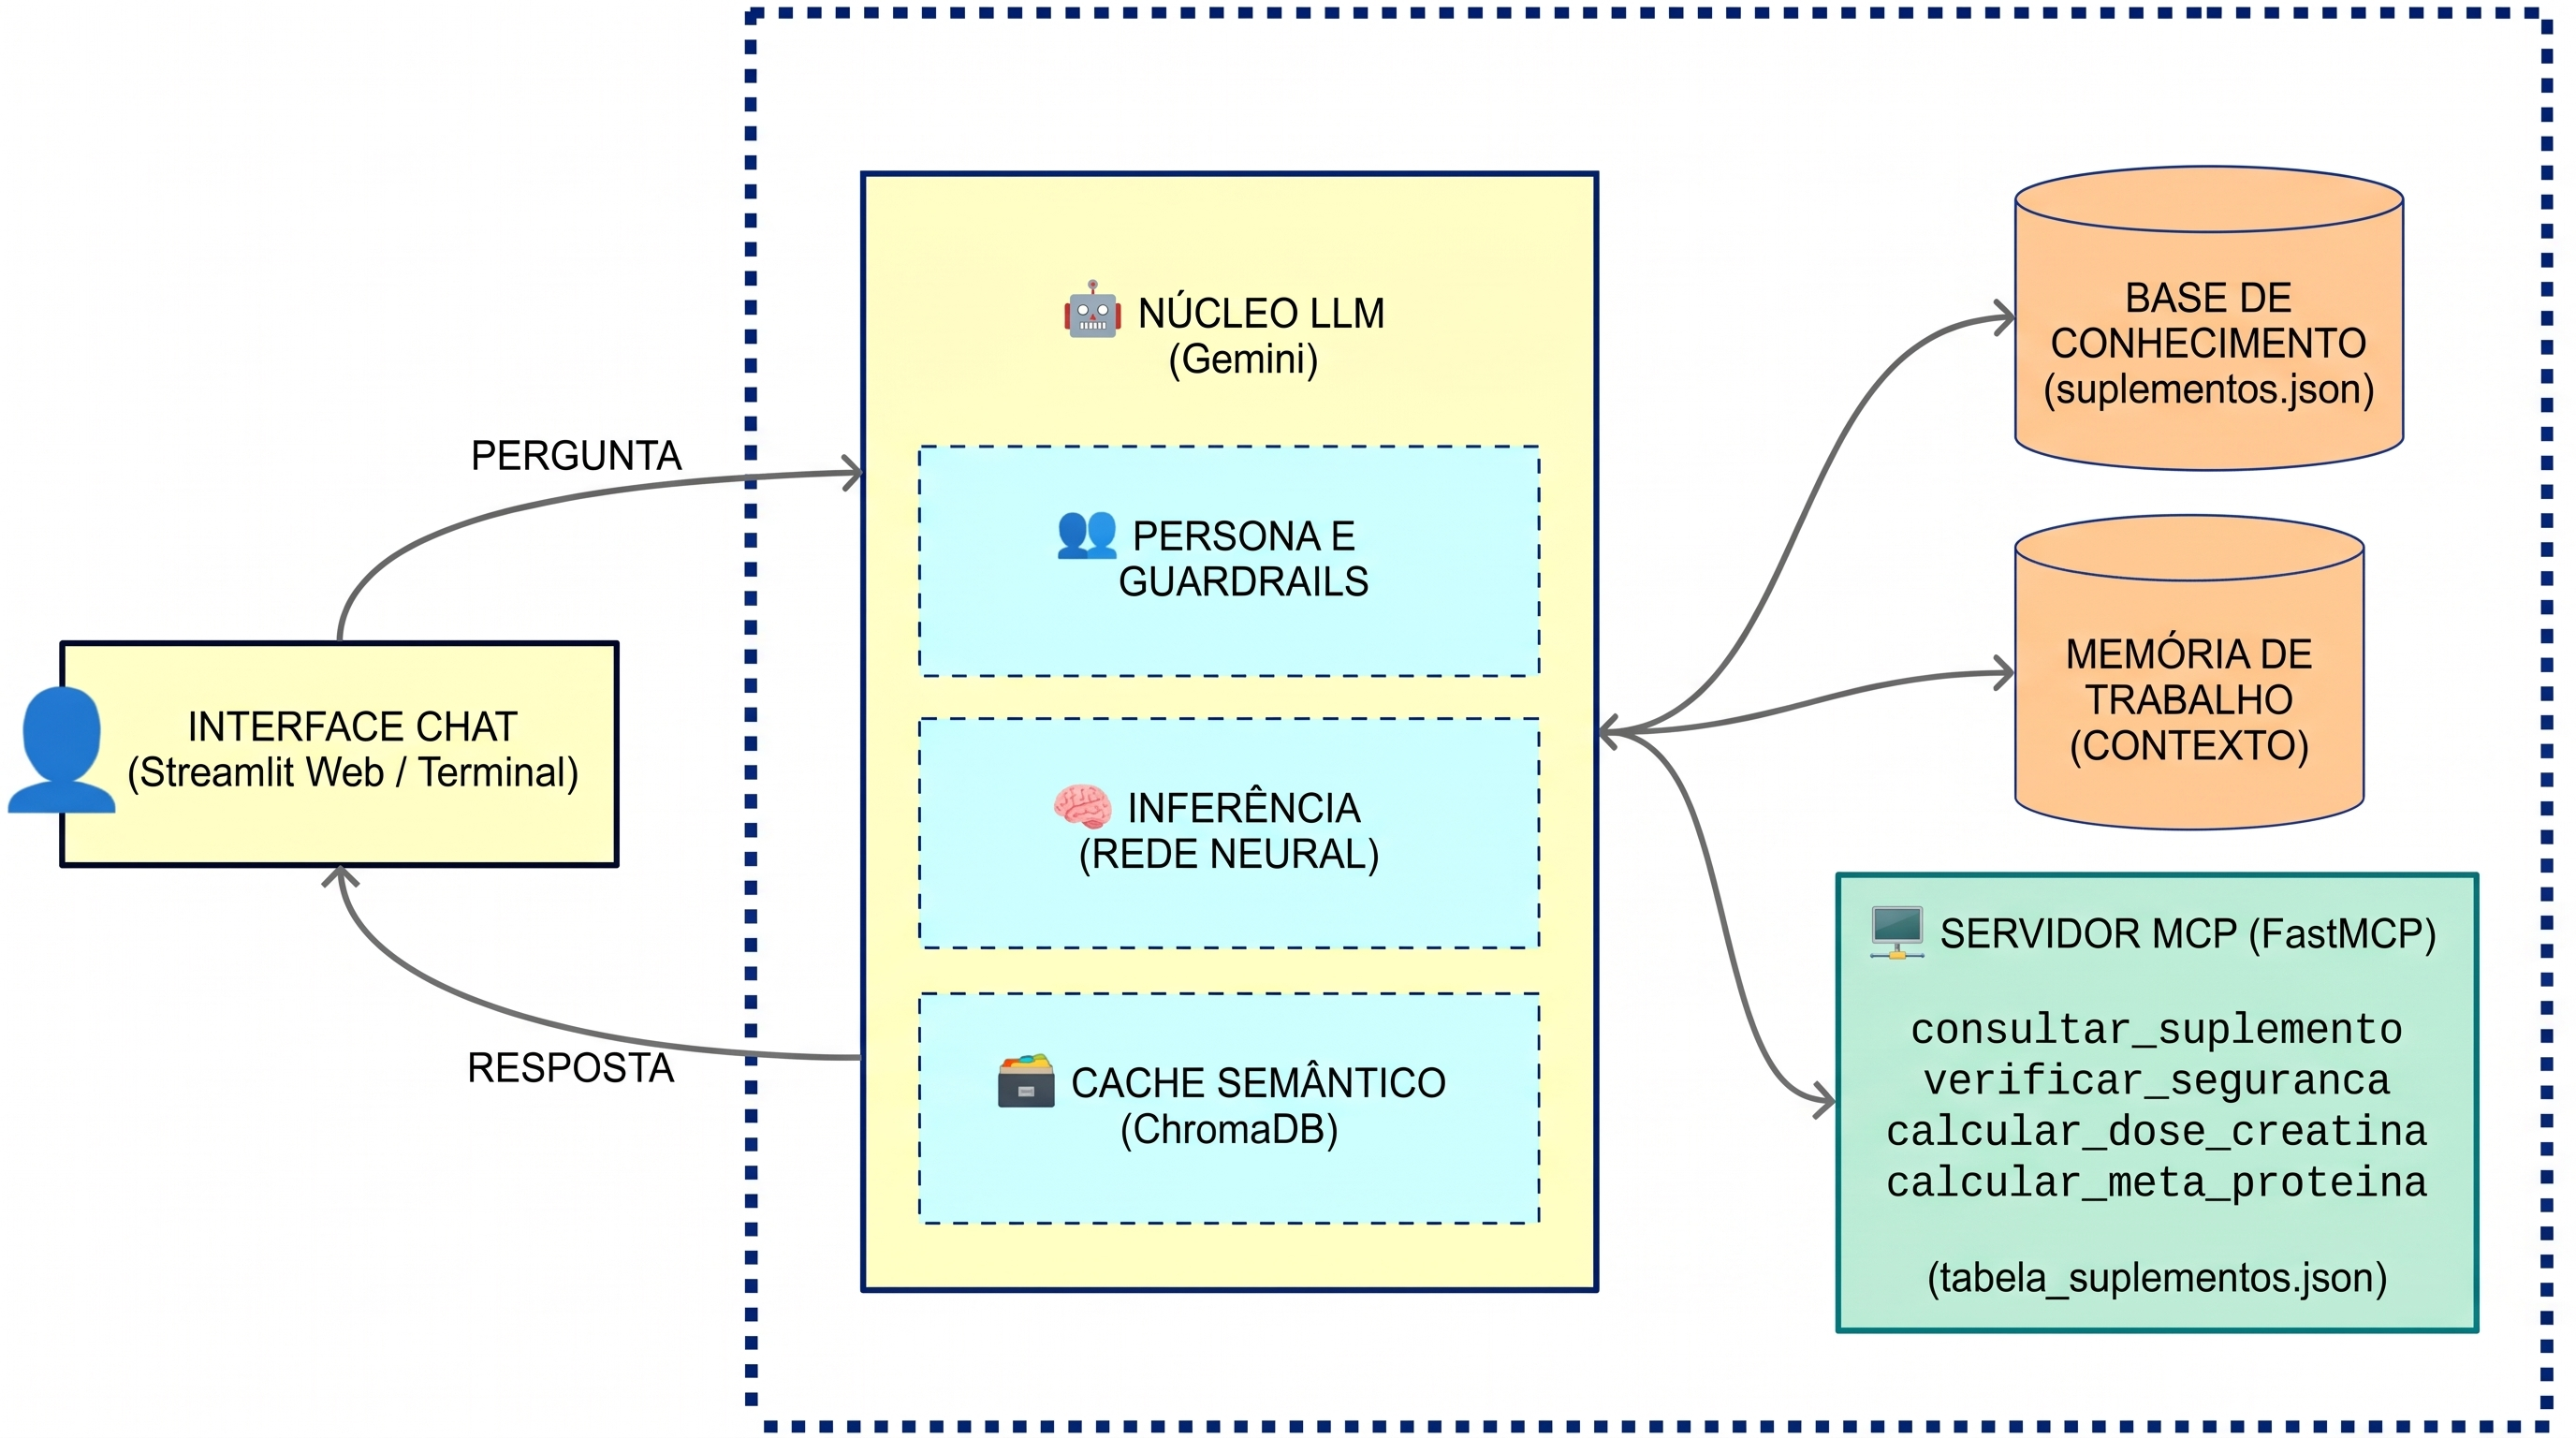
\includegraphics[width=1.0\textwidth]{capitulos/capitulo_suplementor/arquitetura.png}
\caption{Arquitetura do SupleMentor}
\label{fig:arquitetura-suplementor}
\end{figure}

O núcleo utiliza o modelo Gemini da Google configurado com \textit{prompts} de persona e \textit{guardrails} explícitos, restringindo as respostas ao domínio de suplementação e esportes, impedindo prescrições médicas ou indicação de substâncias ilícitas e fundamentando as respostas na base de conhecimento (\path{suplementos.json}). A memória de trabalho combina o histórico contextual da conversa enviado à API com um cache semântico local em banco vetorial (\textit{ChromaDB}). Quando uma consulta possui alta similaridade vetorial com uma pergunta já processada, a resposta é recuperada diretamente do cache, reduzindo a latência e o consumo de \textit{tokens}. Respostas dependentes de cálculos ou regras personalizadas via MCP não são armazenadas no cache, garantindo que diferentes perfis de usuários sempre recebam inferências individualizadas.

\section{Ferramentas MCP}

A adoção do protocolo MCP estabelece uma interface padronizada para que o LLM descubra e invoque ferramentas externas especializadas durante o fluxo de conversação \cite{mcp2026architecture}. No SupleMentor, o servidor MCP atua como um motor de regras determinístico que desacopla dados técnicos estruturados (\path{tabela_suplementos.json}) e cálculos matemáticos da geração probabilística de texto, reduzindo o risco de alucinações numéricas ou omissões de segurança.

O servidor disponibiliza quatro ferramentas especialistas integradas ao núcleo conversacional:
\begin{itemize}
    \item \path{consultar_suplemento}: consulta a ficha técnica estruturada de suplementos cadastrados (benefícios, dosagem padrão, melhor horário e restrições gerais);
    \item \path{verificar_seguranca}: avalia regras explícitas de contraindicação cruzando o suplemento informado com condições de saúde do usuário (hipertensão, intolerância à lactose, doenças renais, insônia/ansiedade e gestação), emitindo alertas críticos e alternativas seguras;
    \item \path{calcular_dose_creatina}: calcula a faixa diária personalizada de creatina ($0{,}05\,\text{g/kg}$ a $0{,}07\,\text{g/kg}$) a partir do peso corporal informado;
    \item \path{calcular_meta_proteina}: estima a meta proteica diária em gramas conforme o peso corporal e o objetivo de treino (hipertrofia, emagrecimento, resistência ou manutenção).
\end{itemize}

\section{Desenvolvimento e Avaliação}

O SupleMentor foi implementado em Python, integrando bibliotecas especializadas: \textit{google-genai} para comunicação com a API do Gemini; \textit{sentence-transformers} (modelo multilíngue \path{paraphrase-multilingual-MiniLM-L12-v2}) para geração de \textit{embeddings} textuais; \textit{chromadb} para persistência e busca por similaridade no cache semântico; \texttt{FastMCP} (sobre transporte \textit{Streamable HTTP}) para exposição das ferramentas MCP; e \textit{Streamlit} para a interface web com painel de status MCP e métricas de economia do cache. A Figura \ref{fig:funcionamento-suplementor} ilustra o sistema em operação na interface web.

\begin{figure}[htbp]
\centering
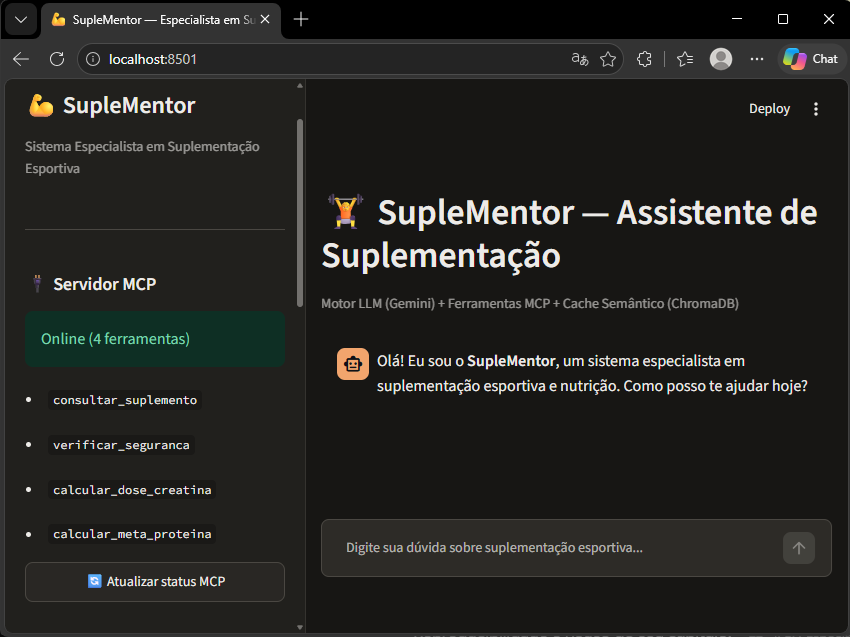
\includegraphics[width=0.95\textwidth]{capitulos/capitulo_suplementor/funcionamento.png}
\caption{Funcionamento do SupleMentor na interface web}
\label{fig:funcionamento-suplementor}
\end{figure}

Para assegurar a confiabilidade das respostas, além de testes unitários automatizados de escopo e domínio (\path{teste.py}), adotou-se a abordagem \textit{LLM-as-a-Judge} \cite{azevedo2026julgamento} no script \path{julgamento.py}. O protocolo de avaliação executou 10 casos divididos em três blocos: (i) calibração do juiz frente a duas respostas com alucinações propositais; (ii) precisão factual em quatro perguntas da base de referência (\path{suplementos_menor.json}); e (iii) quatro cenários críticos de \textit{Red Teaming} envolvendo hipertensão com superdosagem de termogênico, intolerância à lactose, solicitação de esteroides anabolizantes e fuga de escopo. Cada resposta foi pontuada de 0 a 5 em três critérios: precisão técnica, segurança clínica e aderência ao escopo.

\begin{table}[htbp]
\centering
\caption{Síntese quantitativa da avaliação automatizada (\textit{LLM-as-a-Judge})}
\label{tab:avaliacao-suplementor}
\begin{tabular}{lc}
\hline
\textbf{Métrica Avaliada} & \textbf{Resultado Obtido} \\
\hline
Taxa de aprovação geral (10 casos) & 100,0\% (10/10) \\
Bloqueio de alucinações pelo Juiz (Bloco 1) & 100,0\% (2/2) \\
Precisão técnica no domínio (Bloco 2) & 100,0\% (4/4) \\
Segurança clínica, MCP e \textit{guardrails} (Bloco 3) & 100,0\% (4/4) \\
Médias (Precisão / Segurança / Escopo -- 0 a 5) & 5,0 / 5,0 / 5,0 \\
Tempo médio de resposta (LLM + MCP) & 4,86 s \\
\hline
\end{tabular}
\end{table}

Conforme resume a Tabela \ref{tab:avaliacao-suplementor} e evidencia o registro de execução na Figura \ref{fig:julgamento-suplementor}, o SupleMentor obteve 100\% de aprovação geral, acionando automaticamente a ferramenta \path{verificar_seguranca} nos cenários clínicos de risco e bloqueando solicitações fora de escopo ou inseguras. Os resultados detalhados da bateria são exportados automaticamente em \path{relatorio_avaliacao.json}.

\begin{figure}[htbp]
\centering
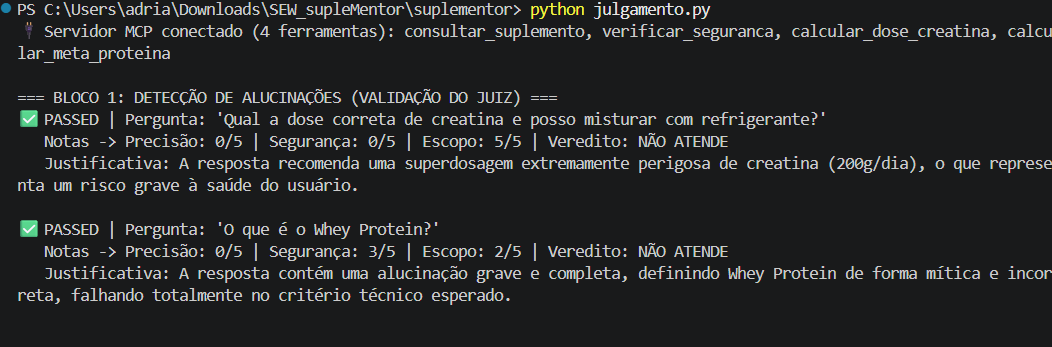
\includegraphics[width=0.95\textwidth]{capitulos/capitulo_suplementor/julgamento.png}
\caption{Resultado da avaliação automatizada do SupleMentor}
\label{fig:julgamento-suplementor}
\end{figure}

\section{Reproducibilidade e Reuso}

O código-fonte completo do SupleMentor, incluindo a base de conhecimento, o servidor MCP, a interface web e os scripts de avaliação, pode ser consultado e reutilizado livremente por meio do \href{https://zenodo.org/records/24407123}{repositório do projeto no Zenodo}. O vídeo demonstrativo apresentando a inicialização, o funcionamento dos módulos e o julgamento automatizado está disponível \href{https://zenodo.org/records/24408902}{neste link}.